\section{Density computations}
* now we choose a different ansatz \\
* instead of obtaining a density field in the form of heatmaps from monte carlo simulations, we aim to compute the density distribution function that holds the particle distribution for $N \rightarrow \infty$ particles \\
* explain what is $\mu^N$, define it \\
The empirical measure $\mu^N$ is the starting point of this computation. 
We define it as:  
\begin{align*}
    \mu^{N}: \mathcal{B}(\R^d) \rightarrow [0,1] \in \mathcal{P}(\R^{dN}) \\
    \mu^{N}(\vec{X}) = \frac{1}{N} \sum\limits_{i=1}^{N} \delta_{\vec{x}_i(t)}.
\end{align*}
% explain dirac, what it does in integrals 
In other words, for a set $A \in \mathcal{B}(\R^d)$, that is a subset of our operating domain, $mu^{N}(A)$ is the relative number of the $N$ particles that are located in $A$. 
For an finite $N \in \N$, $\mu^{N}$ is a discrete measure that only has its mass divided on the exact particle locations. 
As we increase the number of particles, $\mu^{N}$ will spread out \,-\, having more particle locations to cover with each particle having a lower influence on the result of $\mu^{N}$ as we divide through $N$.
This process is quite simular to the transition from a sum to an according integral:
\[ \sum\limits_{i=1}^{N} \frac{1}{N} f(x_i) \xrightarrow{N \to \infty} \int f(x) \dequ x,  \]
where we can also see a transition from a discrete starting problem, having discrete points ${x_i}$, to a continious integral where $x \in (a,b)$. 
As $\mu^N$ is a measure that lives on sets $A \in \mathcal{B}(\R^d)$, we cannot directly plot it as a function. 
Instead, we try to visualise it meaningfully by using histograms as approximations.
This is also a good connection from the previus section, where we also used histograms to show the results of the monte carlo simulations. 

% TODO: add a figure that tries to visualise the transition as N -> infty (just use my heatmaps with 1 simulation and different amounts of particles, colorschale) 
\begin{figure}
	\begin{center}
		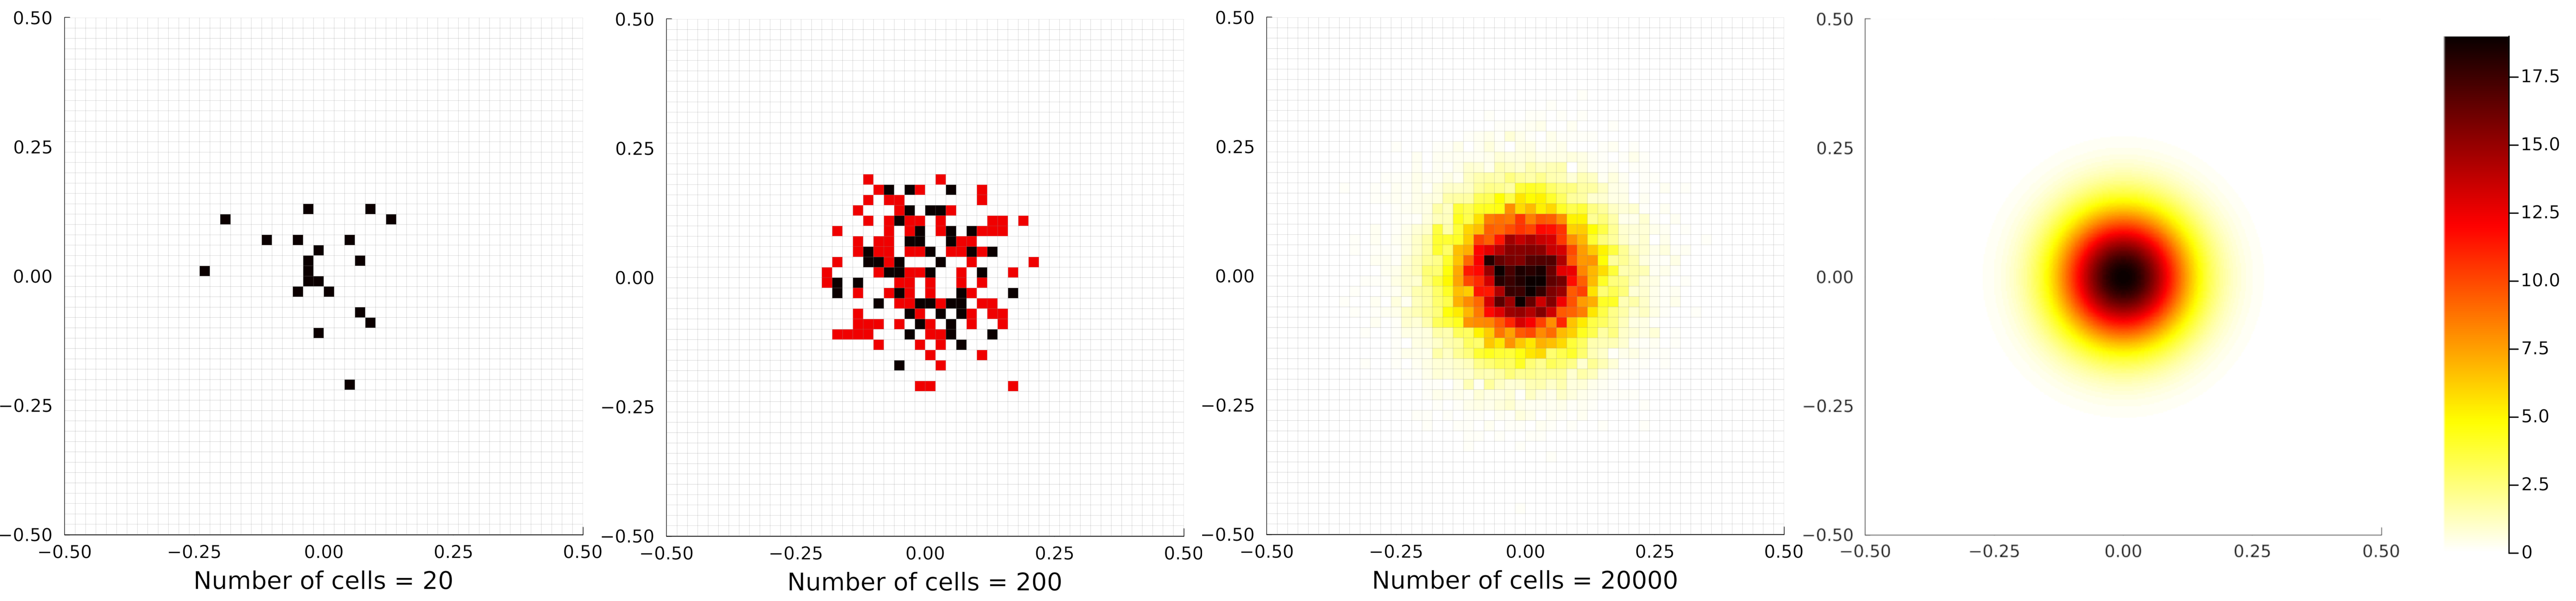
\includegraphics[width=15cm]{density/muplot_combined.png}
		\caption{
            Visualisation of empirical measures $\mu^N$ for increasing numbers of cells, alongside the corresponding theoretical density. 
            This visualisation illustrates the transition \( \mu^N \xrightarrow{N \to \infty} \mu\). \\
            All cell configurations are sampled from the same initial condition described in the previous chapter: a two-dimensional normal distribution \( \mathcal{N}_2((0,0), \sigma^2 I_2) \) with \( \sigma = 0.09 \). 
            In the first three subplots, the domain \([-0.5, 0.5]^2\) is discretised into square bins of side length \(\frac{1}{50}\). 
            Each bin \( A \) corresponds to a measurable set in the definition of the empirical measure \( \mu^N(A) = \frac{1}{N} \sum_{i=1}^N \delta_{x_i}(A) \), where the color intensity encodes the number of cells in that bin. \\
            The first subplot shows a realisation with \( N = 20 \) cells, the second with \( N = 200 \), and the third with \( N = 20{.}000 \). 
            We observe that as \( N \) increases, the empirical measure \( \mu^N \) becomes a smoother approximation of the underlying density. 
            The color scale is fixed across all subplots to allow direct visual comparison.
            The fourth panel displays the exact density function of the initial distribution, \( \rho(x) = \frac{1}{2\pi\sigma^2} \exp\left( -\frac{\|x\|^2}{2\sigma^2} \right) \), with \( \sigma = 0.09 \). 
         }
		\label{fig:muTransition}
	\end{center}
\end{figure}

The distribution from the fourth subplot in Figure~\ref{fig:muTransition} is aimed to be computed for the dynamics of our DF cell model. 

In the end, we want to achieve:
\[ \mu^N \xrightarrow{N \to \infty} \mu\]
by letting the number of cells go to infinity. \\

\subsection{Transition $\mu^N \xrightarrow{N \to \infty} \mu$ }


\subsection{General energy computation}

Let:
\begin{gather*}
    \vec{X} = (\vec{x}_1, \ldots, \vec{x}_d) \in \R^{dN} \\
    \text{for } \vec{x}_i \in \R^d, \; 1 \leq i \leq N, \\
    E: \R^d \rightarrow \R \\ 
    E(\vec{x}_i) = \frac{1}{2} |\vec{x}_i|^2.
    \nabla_{(\vec{x}_i)} E(\vec{x}_i): \R^d \rightarrow \R^d
\end{gather*}

We define the dynamic of a particle $\vec{x}_i$ via: \\
\[ \dfrac{\dequ \vec{x}_i}{\dequ t} = - \nabla_{\vec{x}_i} E(\vec{x}_i) \in \R^{d}. \]

We define the probability measure:\\
(question: is $\mu$ defined on a single particle [$\mu^{N} \in \mathcal{P}(\R^d)$] or on the whole particle system [$\mu^{N} \in \mathcal{P}(\R^{dN})$]) \\
(question: what does $\mu$ say? \\
Its 1 when the particle is at a given location? vs Its 1 when the particle system is at a given configuration?)

\[ \mu: \R^d \rightarrow [0,\infty)  \]
$\mu$ is the density of cell system.
$\mu^N$ is the empirical measure. 
It takes a subset $A \subset \R^d$ as an argument and gives the relative number of particles that are inside of $A$. 

Let $\phi \in C_c^{\infty}(\R^{d}, \R)$ (??) be a test function. 
Its gradient field is $ \nabla \phi : \R^d \rightarrow \R^d$. 
We compute: 
\begin{align*}
    \frac{\dequ}{\dequ t} \int \phi \dequ \mu^N 
    &= \frac{\dequ}{\dequ t} (\frac{1}{N} \sum\limits_{i=1}^{N} \phi(\vec{x}_i)) \\
    &= - \frac{1}{N} \sum\limits_{i=1}^{N} \nabla \phi(\vec{x}_i) \cdot \nabla E(\vec{x}_i) \\
    &= - \frac{1}{N} \sum\limits_{i=1}^{N} \int \nabla \phi(x) \cdot \nabla E(x) \dequ \delta_{\vec{x}_i} \\
    &= - \int \nabla \phi(x) \cdot \nabla E(x) \dequ \mu^N \dequ x \\
    &= \int \phi(x)  \nabla \cdot ( \mu^N(\nabla E(x))) \dequ x \\
\end{align*}
\[ \Rightarrow  0 = \partial_t \rho - \nabla(\rho_v),\]
where $\rho$ is the density function of $\mu$ such that \[ \mu(dx) = \rho(x) dx. \]
question: what is the space we integrate above? (i gues $\R^{dN}$)